%\begin{appendices}
\appendix
\chapter{Weitere Abbildungen und Tabellen}
\label{appendix:abb_tab}
\begin{figure}[h!]
    \centering
    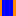
\includegraphics[scale=10]{images/2-1_chroma_artefacts_original.png}
    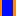
\includegraphics[scale=10]{images/2-1_chroma_artefacts_sampled.png}
    \caption{Artefakte durch Chroma Subsampling}
    \textit{Links: Original, Rechts: Subsampled. Die rechte Kante des blauen Farbblocks liegt in gesubsampleten 2x2 Blöcken, wodurch Artefakte entstehen. Die linke Kante liegt zwischen zwei 2x2 Blöcken, weshalb es zu keiner falschen Darstellung kommt.}
    \label{fig:chroma_artefacts}
\end{figure}

\begin{figure}[h!]
    \centering
    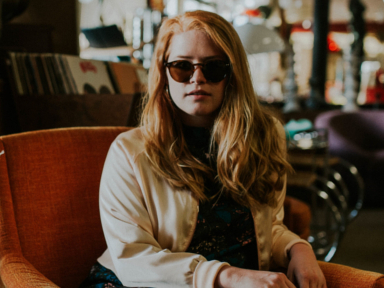
\includegraphics[scale=0.5]{images/2-3_brook_orig.png}
    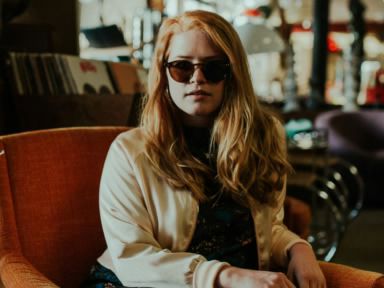
\includegraphics[scale=0.5]{images/2-3_brook_1.png}
    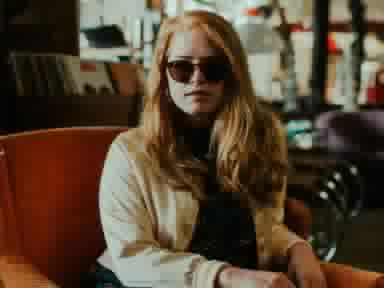
\includegraphics[scale=0.5]{images/2-3_brook_16.png}
    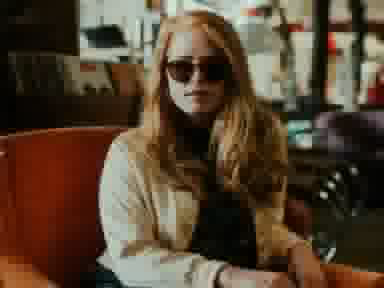
\includegraphics[scale=0.5]{images/2-3_brook_31.png}
    \caption{Ergebnis der Quantisierung mit verschiedenen Quantisierungsfaktoren}
    \textit{Oben links: Original, Oben rechts: Quantisiert mit Faktor 1, Unten links: Quantisiert mit Faktor 16, Unten rechts: Quantisiert mit Faktor 31.\\
    Mit zunehmendem Quantisierungsfaktor ist ein ansteigender Verlust der Bildqualität zu beobachten, wobei grobe Strukturen weitestgehend erhalten bleiben. Original nach \cite{brooke_cagle__2016}}
    \label{fig:quantization_multi_mquants}
\end{figure}

\begin{table}[h!]
\centering
\begin{tabular}{|c|c|c|c|c|c|c|c|}
	\hline
	8 & 16 & 19 & 22 & 26 & 27 & 29 & 34 \\
	16 & 16 & 22 & 24 & 27 & 29 & 34 & 37 \\
	19 & 22 & 26 & 27 & 29 & 34 & 34 & 38 \\
	22 & 22 & 26 & 27 & 29 & 34 & 37 & 40 \\
	22 & 26 & 27 & 29 & 32 & 35 & 40 & 48 \\
	26 & 27 & 29 & 32 & 35 & 40 & 48 & 58 \\
	26 & 27 & 29 & 34 & 38 & 46 & 56 & 69 \\
	27 & 29 & 35 & 38 & 46 & 56 & 69 & 83 \\
	\hline
\end{tabular}
\caption{Voreingestellte MPEG-1 Intracoding Quantisierungsmatrix. \cite{symes_peter_digital_2004} }
\label{tab:default_quant}
\end{table}

%\end{appendices}
